% $Header: /cvsroot/latex-beamer/latex-beamer/solutions/generic-talks/generic-ornate-15min-45min.en.tex,v 1.5 2007/01/28 20:48:23 tantau Exp $
\documentclass{beamer}
\mode<presentation>
{
 \usetheme{Warsaw}
 \usecolortheme{beaver}
 \usecolortheme{rose}
 \setbeamercovered{transparent}
}
\usepackage[english]{babel}
\usepackage[latin1]{inputenc}
\usepackage{graphicx}
\usepackage{times}
\usepackage[T1]{fontenc}

\title{Cloud Computing and the Ideal Mobile Platform}
\subtitle{How the advent of Cloud Computing might affect computers designed for
  mobile use}
\author{T.~Visher}
\institute[Chestnut Hill College]{Department of Computer Science\\
  Chestnut Hill College}
\date[Senior Seminar]{May 3rd, 2010 / Senior Seminar Presentation}
\subject{Cloud Computing and the Ideal Mobile Platform}

\pgfdeclareimage[height=0.75cm]{chc-logo}{redgrif}
\logo{\pgfuseimage{chc-logo}}

% Delete this, if you do not want the table of contents to pop up at
% the beginning of each subsection:
\AtBeginSubsection[]{
  \begin{frame}<beamer>{Outline}
    \tableofcontents[currentsection,currentsubsection]
  \end{frame}
}

\begin{document}

\begin{frame}
\titlepage
\end{frame}

\begin{frame}{Outline}
\tableofcontents[pausesections]
% You might wish to add the option [pausesections]
\end{frame}

% Since this a solution template for a generic talk, very little can
% be said about how it should be structured. However, the talk length
% of between 15min and 45min and the theme suggest that you stick to
% the following rules:

% - Exactly two or three sections (other than the summary).
% - At *most* three subsections per section.
% - Talk about 30s to 2min per frame. So there should be between about
%   15 and 30 frames, all told.

\section[Introduction]{Research Questions and Goals}

\begin{frame}{Goals}

\begin{itemize}
  \item A new mobile machine
  \item Prove Netbook/Notebook comparability
\end{itemize}

\end{frame}

\begin{frame}{Research Questions}
  \begin{itemize}
  \item Can the use of Cloud Services extend battery life?
  \item Are Netbooks and Notebooks favorably comparable \\ in the use of Cloud
    Services?
  \end{itemize}
\end{frame}

\section[Literature Review]{The Literature: The Internet and Computing}

\subsection{Thin Client Computing}

\begin{frame}{History}
  \begin{itemize}
  \item Client/Server
  \item Architecture
  \end{itemize}
\end{frame}

\begin{frame}{An Implementation: SLIM}
  \begin{columns}
    \column{5cm}
      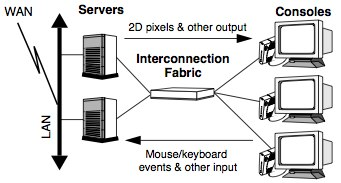
\includegraphics[width=5cm]{slimArchitecture.jpg}
    \column{5cm}
      \begin{itemize}
      \item Sun Microsystems (RIP)
      \item Architecture
      \item Rationale
      \end{itemize}
  \end{columns}
\end{frame}

\begin{frame}{Why?}
  \begin{itemize}
  \item Advantages
  \item Disadvantages
  \end{itemize}
\end{frame}

%% \begin{frame}{Current Applications}
%%   \begin{itemize}
%%   \item Medical Industry
%%   \end{itemize}
%% \end{frame}

\subsection{Cloud Computing}

\begin{frame}{History}
  \begin{itemize}
  \item Roots
  \item Amazon
  \item Broadband
  \end{itemize}
\end{frame}

\begin{frame}{Web 2.0}
  \begin{itemize}
  \item Tim O'Reilly
  \item Ethos
  \item Examples
  \end{itemize}
\end{frame}

\subsection{Netbooks and Ultra-Mobile PCs}

\begin{frame}{History}
  \begin{columns}
    \column{5cm}
      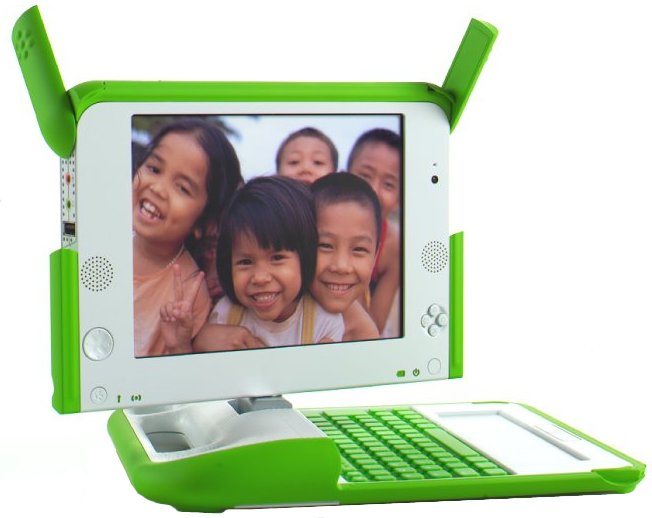
\includegraphics[width=5cm]{olpc.jpg}
    \column{5cm}
      \begin{itemize}
      \item Intel %% Paul Bergevin, 2008
      \item The First Netbook
      \item Drivers
      \end{itemize}
  \end{columns}
\end{frame}

\begin{frame}{Qualifications}
  \begin{columns}
    \column{5cm}
      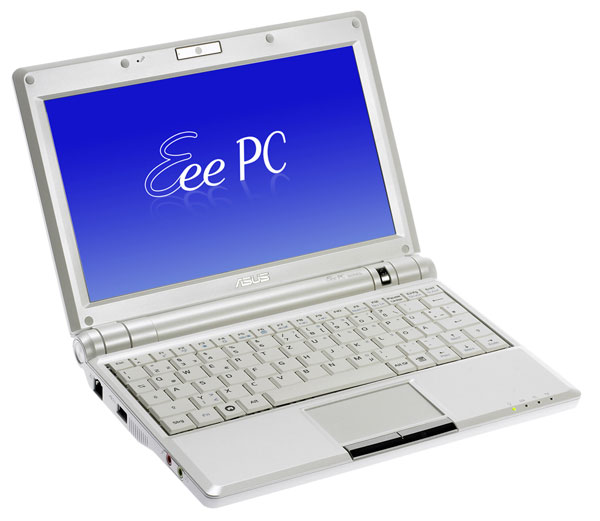
\includegraphics[width=5cm]{netbookSpecs.jpg}
    \column{5cm}
      \begin{itemize}
      \item Small
      \item Cheap
      \item Depend on the Net
      \end{itemize}
  \end{columns}
\end{frame}

\subsection{Lithium-Ion Batteries}

\begin{frame}{History}
  \begin{columns}
    \column{5cm}
      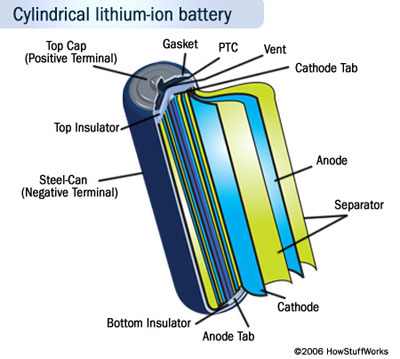
\includegraphics[width=5cm]{lionSummary.jpg}
    \column{5cm}
      \begin{itemize}
      \item Prior Art
      \item Exxon % M. S. Whittingham, 1976
      \item Safety
      \end{itemize}
  \end{columns}
\end{frame}

\begin{frame}{How They Work}
  \begin{columns}
    \begin{column}{5cm}
      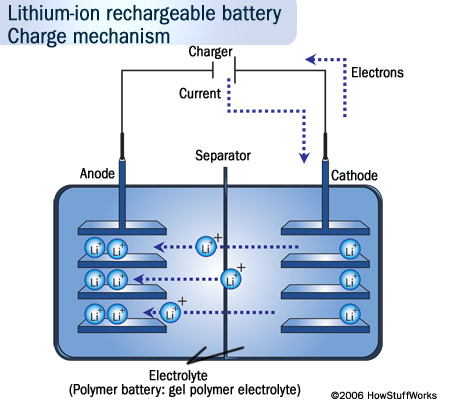
\includegraphics[width=5cm]{lionCharge.jpg}
    \end{column}
    \begin{column}{5cm}
      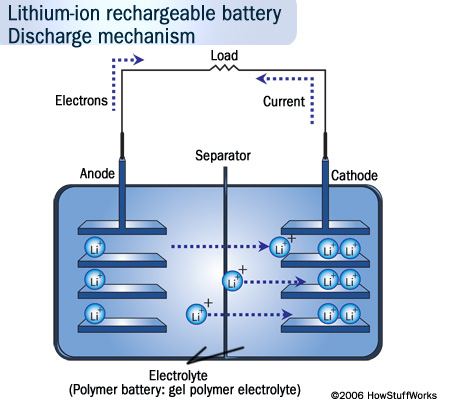
\includegraphics[width=5cm]{lionDischarge.jpg}
    \end{column}
  \end{columns}
\end{frame}

\begin{frame}{Future Research}
  \begin{itemize}
  \item Nano Technology
  \end{itemize}
\end{frame}

\section[Research Project]{The Project: Demand Management and Google Docs Spreadsheet Torture Test}

\subsection{Demand Management}

\begin{frame}{What Is Demand Management? }
  \begin{columns}
    \column{5cm}
      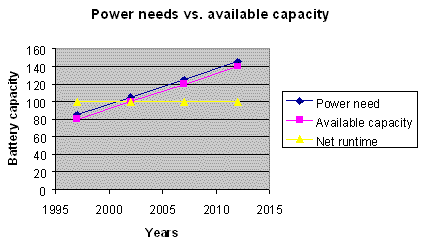
\includegraphics[width=5cm]{demandGraph.png}
    \column{5cm}
    \begin{itemize}
    \item It is\dots
    \item Why?
    \item Mr. Pogue
    \end{itemize}
  \end{columns}
\end{frame}

\begin{frame}{Notebooks+Demand Management}
  \begin{columns}
    \column{5cm}
      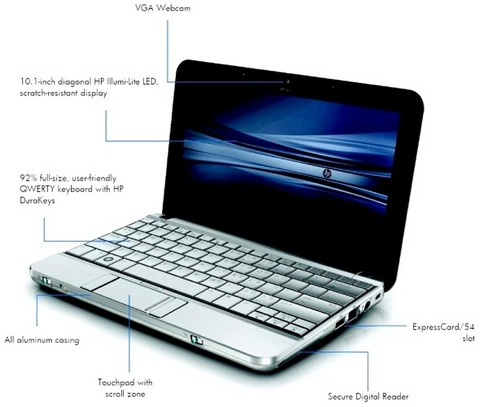
\includegraphics[width=5cm]{netbookDiagram.jpg}
    \column{5cm}
    \begin{itemize}
    \item Display Size
    \item Antenna Switch
    \item SSD
    \item CPU Throttling
    \item No Optical
    \end{itemize}
  \end{columns}
\end{frame}

\subsection[GDocs Spreadsheet Testing]{Google Docs Spreadsheet Torture Test}

\begin{frame}{Make Titles Informative.}
\end{frame}

\section*{Summary}

\begin{frame}{Summary}

\begin{itemize}
  \item The \alert{first main message} of your talk in one or two lines.
  \item The \alert{second main message} of your talk in one or two lines.
  \item Perhaps a \alert{third message}, but not more than that.
\end{itemize}

\end{frame}

\begin{frame}{Future Research}
% The following outlook is optional.
\begin{itemize}
  \item Outlook
  \begin{itemize}
    \item Something you haven't solved.
    \item Something else you haven't solved.
  \end{itemize}
  \end{itemize}
\end{frame}

\end{document}
